\documentclass[10pt]{article}
\usepackage[utf8]{inputenc}
\usepackage[T1]{fontenc}
\usepackage[italian]{babel}

\usepackage{geometry}
\geometry{a4paper}

\usepackage{fancyhdr}
\pagestyle{fancy}
\renewcommand{\headrulewidth}{0pt}
\lhead{}\chead{}\rhead{}
\lfoot{}\cfoot{\thepage}\rfoot{}

\usepackage{graphicx}
\usepackage{booktabs}
\usepackage{paralist}
\usepackage{verbatim}
\usepackage{subfig}
\usepackage{wrapfig}
\usepackage{pdfpages}

\usepackage{sectsty}

\usepackage[titles,subfigure]{tocloft}
\renewcommand{\cftsecfont}{\rmfamily\mdseries\upshape}


\title{ADC DAC GPIO Board for Raspberry}
\author{Patrick Predella 165283, Federico D'Eredità 151646 }
\date{}

\begin{document}
\maketitle
\tableofcontents

\section{Introduzione}
Finalità del progetto è il monitoraggio di misure di temperatura e pressione ambientali mediante sensoristica analogica con la possibilità di comandare attuatori analogici e/o digitali tramite programmazione di un Raspberry Pi2+.
A questo scopo abbiamo deciso di realizzare una scheda composta dai seguenti elementi principali:
\begin{itemize}
\item Un convertitore analogico-digitale per il campionamento dei segnali analogici di temperatura e pressione affiancato da una protezione per eventuali sbalzi di tensione;
\item Un convertitore digitale-analogico per il controllo di attuatori analogici anch'esso affiancato da una protezione per eventuali sbalzi di tensione;
\item Un general purpose input/output per il controllo di attuatori digitali ed il controllo delle operazioni pre-programmate nel Raspberry;
\item Scheda PiggyBack (vedasi capitolo \ref{sec:piggy}) per l'assemblaggio della componentistica;
\item Un Raspberry Pi2+ per il controllo delle linee dati, di clock e l'interazione con il GPI/O.
\end{itemize}


\section{Componentistica}
	\subsection{Cicuiteria utilizzata}

		\subsubsection{ADC - Analog-to-Digital Converter}\label{sec:adc}
		L'ADC è un dispositivo per la conversione di segnali analogici in segnali digitali, i suoi aspetti più importanti sono risoluzione e frequenza di campionamento.
		La risoluzione è legata al numero di bit di memoria disponibili nel dispositivo e influenza la sua capacità di discernere segnali in ingresso simili tra loro mediante $2^{n-1}$ step di campionamento (con n pari al numeri di bit disponibili). La frequenza di campionamento invece determina in che misura la conversione segua fedelmente l'andamento nel tempo del segnale di ingresso. Come noto dal teorema di Shannon la frequenza di campionamento deve essere almeno più del doppio della frequenza del segnale ingresso, nel caso in esame comunque i segnali di temperatura e pressione essento riferiti a misure ambientali hanno frenquenze molto basse.

		Nel nostro progetto utilizziamo un MCP3428 della Microchip Technology Inc. caratterizzato da una frequenza di lavoro a 100 kHz, 400 kHz o 3.4 MHz (nella nostra applicazione imposteremo 100 kHz) ed una risoluzione a 16bit e 4 canali d'ingresso. In Figura \ref{fig:adc} è possibile vedere una schematizzazione a blocchi del funzionamento dell'ADC in uso ed i suoi pin.
		\begin{figure}[h]
			\centering
			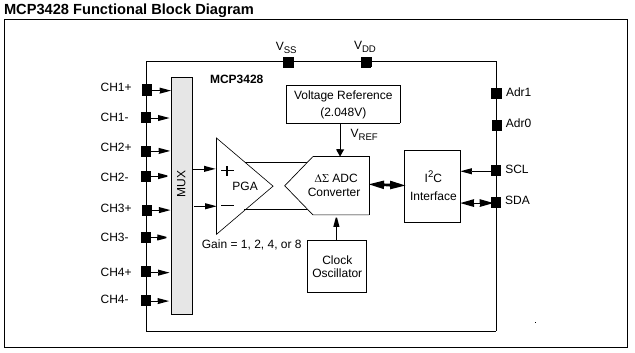
\includegraphics[width=0.8\textwidth]{src/adc_block}
			\caption{Schema a blocchi dell'ADC}\label{fig:adc}
		\end{figure}

		L'MCP3428 dispone di una sua Vref interna, modificabile tramite il settagio del PGA mediante la relazione $V_{ref}=V_{ref-base}/PGA$, nello specifico del nostro progetto impostiamo il PGA (Programmable Gain Amplifier) a 1x.


		\subsubsection{DAC - Digital-to-Analog Converter}\label{sec:dac}
		Il DAC è un dispositivo per la conversione di segnali digitali in segnali analogici, è concettualmente l'opposto dell'ADC visto precedentemente.
		Nel nostro progetto utilizziamo un MCP4728 della Microchip Technology Inc. le cui specifiche tecniche sono comparabili con quelle dell'MCP3428 se non per ilfunzionamento. Dato uno stream di dati in ingresso ne viene ricostruito l'andamento in tensione analogica  mediante un sincronizzatore, quest'ultimo per evitare che la tensione generata abbia un andamento ad impulsi viene affiancato da dei latch di tensione che permettono di realizzare un'andamento continuo di tensione senza sbalzi.
		In Figura \ref{fig:dac} è possibile vedere una schematizzazione a blocchi del DAC in uso ed i suoi pin.
		\begin{figure}[h]
			\centering
			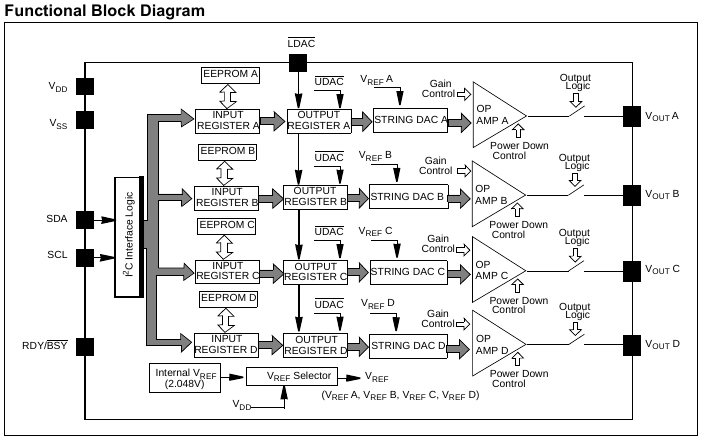
\includegraphics[width=0.8\textwidth]{src/dac_block}
			\caption{Schema a blocchi del DAC}\label{fig:dac}
		\end{figure}

		\subsubsection{GP I/O - General Purpose Input/Output Device}\label{sec:gpio}
		\begin{wrapfigure}{l}{0.3\textwidth}
		\vspace{-20pt}
			\centering
			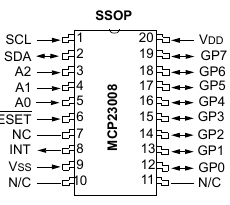
\includegraphics[width=0.3\textwidth]{src/gpio_scheme}
			\caption{Schema del GPIO}\label{fig:gpio}
			\vspace{-10pt}
		\end{wrapfigure}
		Il GP I/O è un dispositivo digitale che dispone di diverse linee che possono fungere sia da canali di input che di output in base ai comandi I\(^2\)C impartiti dal controllore master (nel nostro caso il Raspberry). Il GP I/O permette quindi di trasmettere e ricevere comandi digitali a/da interruttori, attuatori digitali e simili, un esempio pratico può essere il controllo remoto del Raspberry mediante interruttori che possono attivvare/disattivare funzioni pre-programmate, scegliere da quale ADC stare in ascolto, o quale DAC attivare ecc. L'uso di un GP I/O può spaziare a fantasia. Nel nostro progetto utilizziamo un MCP23008 che dispone di 8bit configurabili tramite I\(^2\)C come input/ouput.



\newpage
		\subsubsection{DCDC Converter}\label{sec:dcdc}
		Il DCDC è un componente che converte una tensione in continua in un'altra tensione in continua secondo i suoi parametri di datasheet.
		L'alimentazione verrà formita da un alimentatore da 12VDC. Tuttavia la nostra scheda monta componentistica che richiede una alimentazione a 5VDC. Usiamo quindi un DCDC converter sia per abbassare la tensione a quella desiderata che per eliminare oscillazioni dovute a eventuali picchi in ingresso
		\begin{figure}[h]
			\centering
			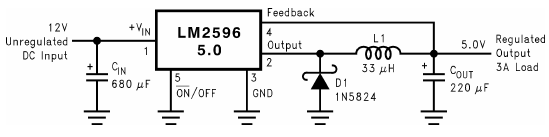
\includegraphics[width=0.8\textwidth]{src/dcdc_scheme}
			\caption{Schema del DCDC completo di filtro stabilizzatore In e Out}\label{fig:dcdc}
		\end{figure}

		Nel nostro progetto utilizziamo un LM2596, un DCDC converter con Vin tra 10V e 40V e Vout stabilizzata a 5V con tolleranza \(<\)0.1\%, più che sufficente per rispettare la compatibilità con gli Absolute maximum ratings dei nostri componenti (5\(\pm\)0.005V).
		L'LM2596 per un'efficace stabilizzazione della tensione in uscita dispone di una closed-loop feedback (nel caso in cui questa sia separata da un filtro per esempio), dispone inoltre di un condensatore in ingresso e un filtro in uscita per smorzare eventuali sovra-tensioni (entranti ed uscenti) evitando quindi glitch nell'alimentazioni dei componenti digitali.

	\subsection{Ulteriori Componenti Hardware}
		\subsubsection{La scheda Piggy-Back}\label{sec:piggy}
	Il Piggy-Back è un semplice accessorio per il Raspberry, è collegabile tramite una porta seriale e fondamentalmente funge da breadboard per il Raspberry. E' infatti su questa scheda dove vengono montati tutti i pezzi fin'ora descritti per analisi di test e collaudo.

		\subsubsection{Il Raspberry}\label{sec:rasp}
	Il Raspberry è un noto microcomputer delle dimensioni di una carta di credito, viene venduto equipaggiato di processore ARMv6/7, scheda grafica e banchi ram integrati. E' un dispositivo poco costoso e di facile impiego per la programmazione di software e circuiti, confidando nella sua notorietà tralasciamo una descrizione più completa e accurata che è comunque disponibile sul sito stesso del produttore.

	\subsection{Il linguaggio di programmazione I2C}\label{sec:i2c}
		I\(^2\)C è l'abbreviazione di \emph{Inter-Integrated Circuit}, più che un vero e proprio linguaggio è un sistema di comunicazione seriale utilizzato tra circuiti integrati. E' caratterizzato dall'uso di sole due linee \emph{SDA} e \emph{SDC} rispettivamente per data e clock, inoltre consente una facile gestione delle linee in \emph{3-state logic} il tutto a scapito di elevate velocità di comunicazione.
		In I\(^2\)C le linee di comunicazione e controllo sono generalmente di tipo \emph{open-drain} rendendo quindi necessario l'uso di resistenze di \emph{pull-up} per la corretta transizione tra i livelli logici alti e bassi.
		In Figura \ref{fig:i2c} una schematizzazione molto ridotta del sistema I\(^2\)C.
		\begin{figure}[h]
		\centering
		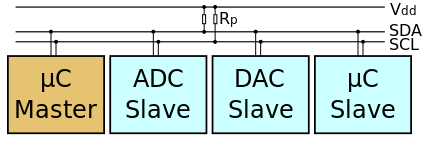
\includegraphics[width=0.5\textwidth]{src/i2c}
		\caption{Schematizzazione I\(^2\)C}\label{fig:i2c}
		\end{figure}


\section{Realizzazione del Progetto}
		Il progetto è molto semplice. Si tratta di:
		\begin{itemize}
		        \item Utilizzare il DCDC converter per stabilizzare l'alimentazione dei componenti;
		        \item Portare le piste a degli header in modo che siano accessibili al Raspberry;
		        \item Proteggere le linee in ingresso e in uscita in modo che non si danneggino i componenti.
		\end{itemize}

	\subsection{Protezione della componentistica}
		Tutti i componenti descritti fin'ora hanno, ovviamente, dei limiti costruttivi sulle tensioni e le correnti che vi possono fluire. Per rientrare nei parametri massimi consentiti (Absolute Maximum Ratings) dobbiamo realizzare delle protezioni sulle linee in ingresso e in uscita da valori \textbf{out of range} e inoltre per \textbf{ridurre i rumori}.
		In particolare realizziamo un filtro per i rumori per l'ADC, un filtro per avere un transitorio non nullo nel caso dei GPIO e per tutti e tre gli integrati (GPIO, ADC e DAC) una protezione contro ingressi troppo alti e per rientrare negli Absolute Maximum ratings nel caso di collegamento dei pin di output a massa (caso peggiore).
		(Vedasi l'appendice corrispondente)

		\subsubsection{Filtri RC}
		Abbiamo disegnato due filtri RC:
		\begin{itemize}
		        \item Un filtro per l'ADC;
		        \item Un filtro per il GPIO.
		\end{itemize}

		Si tratta in entrambi i casi di filtri passa basso ad 1 polo.

			\paragraph{Filtro ADC}
				L'ADC già di per sé secondo le sue specifiche si comporta come un passa basso a 5Hz, nel nostro caso vogliamo aggiungere un ulteriore polo in modo da \textbf{pre-filtrare} il segnale in ingresso.
				Scegliamo quindi una frequenza di taglio \textbf{\(<\)5Hz} (soglia oltre la quale ogni caso il segnale non verrebbe campionato correttamente).
				In particolare scegliamo una resistenza da 100k\(\Omega\) e un condensatore da 1\(\mu\)F per avere di conseguenza un taglio a 1.6Hz.
			\paragraph{Filtro GPIO}
				Per il GPIO il caso è diverso: ci serve un filtro in modo da evitare false letture dovute a picchi improvvisi e rumore e nel contempo asssicurare una buona reattività nel caso dell'attuazione
				Dimensioniamo il filtro a partire dalla resistenza che deve soddisfare la massima corrente di drain dal piedino descritta negli \textbf{Absolute Maximum Ratings}.
				Abbiamo quindi Imax=25mA, Vmax=5V. Rmin deve quindi essere Rmin=200\(\Omega\). La dimensioniamo ad 1k\(\Omega\) e siamo sicuri di essere nei ratings.
				Scegliamo una C=1\(\mu\)F per avere di conseguenza un taglio a 160Hz. La porta ha quindi una \(\tau\)=1ms di risposta naturale, che nella nostra applicazione è accetabile in quanto nel caso peggiore la commutazione del valore binario avviene intorno ai 2ms.
		\subsubsection{Protezioni V e I}
		Ci serve un sistema per impedire alla tensione di salire oltre ad una certa soglia in modo da non danneggiare i microchip. utilizziamo quindi dei diodi Zener che scaricano a massa le tensioni in ingresso.
		Si noti che le usiamo anche nel caso dei DAC per proteggere la porta nel caso in cui venga collegata erroneamente.
			\paragraph{Protezione DAC}
				Nel caso del DAC vogliamo proteggere la porta da tensioni troppo alte. Al massimo il DAC da Vout=Vdd=5V. Colleghiamo un diodo Zener con Vz=5.1V in inversa e qualunque tensione maggiore di 5.1 verrà scaricata dal componente.
				La resistenza viene scelta per rispettare la massima corrente erogata dal pin Imax=25mA. Con V=5V e Imax=25mA, Rmin=200\(\Omega\). La dimensioniamo ad 1k\(\Omega\).
			\paragraph{Protezione GPIO}
				Pure nel caso del GPIO vogliamo proteggere la porta da tensioni troppo alte. Al massimo il GPIO da Vout=Vdd=5V. Colleghiamo un diodo Zener con Vz=5.1V in inversa e qualunque tensione maggiore di 5.1 verrà scaricata dal componente.
				La resistenza viene scelta per rispettare la massima corrente erogata dal pin Imax=25mA. Con V=5V e Imax=25mA, Rmin=200\(\Omega\). La dimensioniamo ad 1k\(\Omega\).
			\paragraph{Protezione ADC}
				Nel caso dell'ADC vogliamo proteggere la porta da tensioni troppo alte. I max ratings sono a 5V, ma qualunque segnale con tensione maggiore di Vref non viene campionato correttamente,
				infatti abbiamo un fenomeno di clipping a V\(<\)-Vref/PGA e a V\(>\)Vref/PGA. (con PGA = 1,2,4,8).
				L'intervallo utile su cui misurare il segnale sono quindi delle tensioni con la tensione -2.048V\(<\)\textbf{V}\(<\)2.048V.

				Colleghiamo un diodo Zener con Vz=2.2V in inversa e in modo da evitare questo compito al microchip.
				In questo caso la resistenza viene scelta per rispettare la massima corrente erogata, ma anche per scegliere condensatori più piccoli e quindi meno costosi.
				La dimensioniamo ad 100k\(\Omega\). Per usare un C=1\(\mu\)F. In ogni caso i segnali che leggeremo trasportano pochissima corrente, quindi possiamo filtrare la corrente massima molto pesantemente.


	\subsection{Specifiche da rispettare per il bus I\(^2\)C}

		Il bus I\(^2\)C richiede pochissime specifiche: una tensione e una frequenza di funzionamento.
		Nel nostro caso dobbiamo solamente scegliere la corretta resistenza di pull-up per la frequenza di funzionamento del bus.
		In particolare utilizzeremo la velocità di trasmissione standard a 100kbit/s.
		Per lo standard I\(^2\)C i bus di default devono essere di tipo \emph{open-drain}, quindi normalizzati a Vdd. Serve quindi una R cosiddetta di pull-up che in un transitorio circa uguale alla durata di 1 ciclo di clock riporti la tensione da gnd a Vdd.
		Lo standard suggerisce che per pochi componenti sullo stesso bus, a velocità standard, una resistenza di 10K\(\Omega\) sia compatibile.
		Utilizziamo quindi resistenze da 10K\(\Omega\).

		Il Raspberry ha già integrate delle resistenze di pull-up per il caso in cui lo si colleghi in I\(^2\)C ad altri componenti.
		Nel caso in cui il segnale sia più pulito con l'alimentazione del bus provvista dal Raspberry, sarà sufficiente dissaldare le R\_pullup e il bus sarà scollegato dalla Vdd fornita dal DCDC.

\newpage
\newgeometry{top=1.5cm,bottom=1.5cm}
	\subsection{Schema elettrico d'assemblaggio}
	\begin{figure}[h!]
		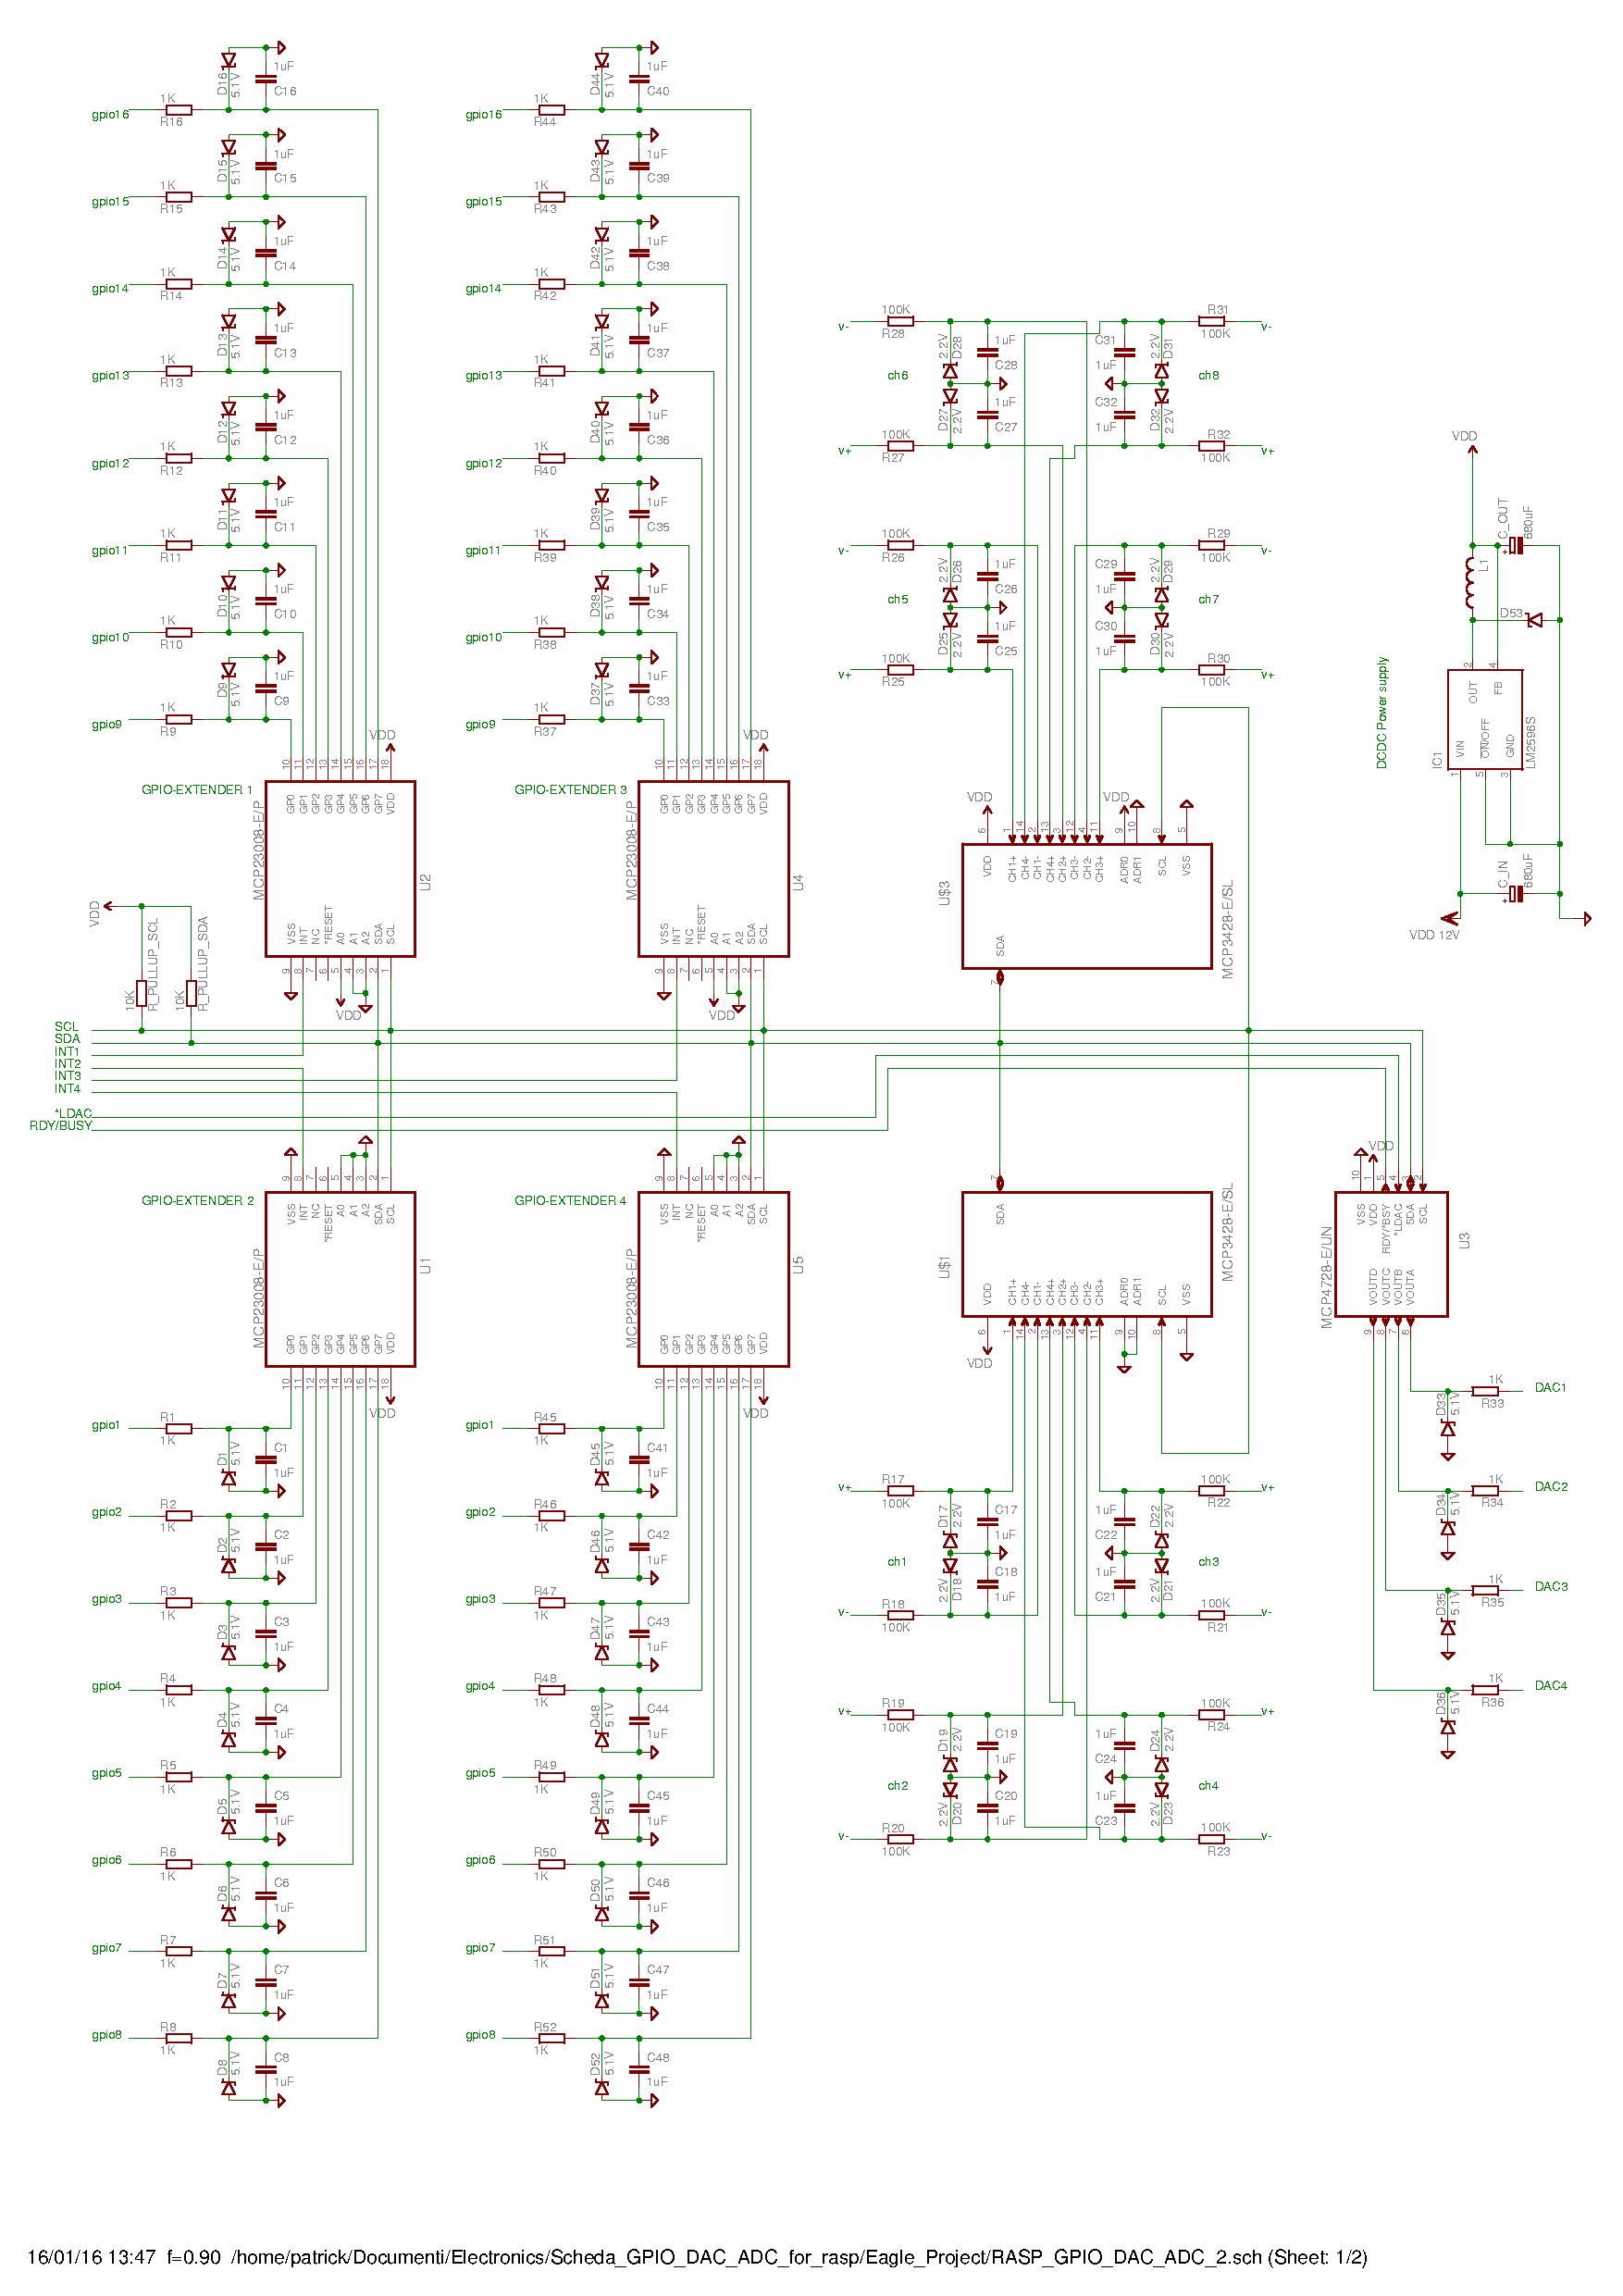
\includepdf[scale=0.9, offset=0 -15]{../PDF_generated/RASP_GPIO_DAC_ADC_2}
	\end{figure}
\restoregeometry

\section{Appendice}
\subsection{Appendice A - Scheda tecnica ADC}
		\includepdf[pages={5},noautoscale=true, offset=0 0]{../Specs/MCP3428}

\newpage
\subsection{Appendice B - Scheda tecnica DAC}
		\includepdf[pages={3},noautoscale=true, offset=0 0]{../Specs/MCP4728}

\newpage
\subsection{Appendice C - Scheda tecnica GPIO}
	\includepdf[pages={23},noautoscale=true, offset=0 0]{../Specs/MCP23008}

\newpage
\subsection{Appendice D - Scheda tecnica DCDC}
	\includepdf[pages={2},noautoscale=true, offset=0 0]{../Specs/LM2596}

\newpage
\subsection{Appendice E - Eagle Project parts}
	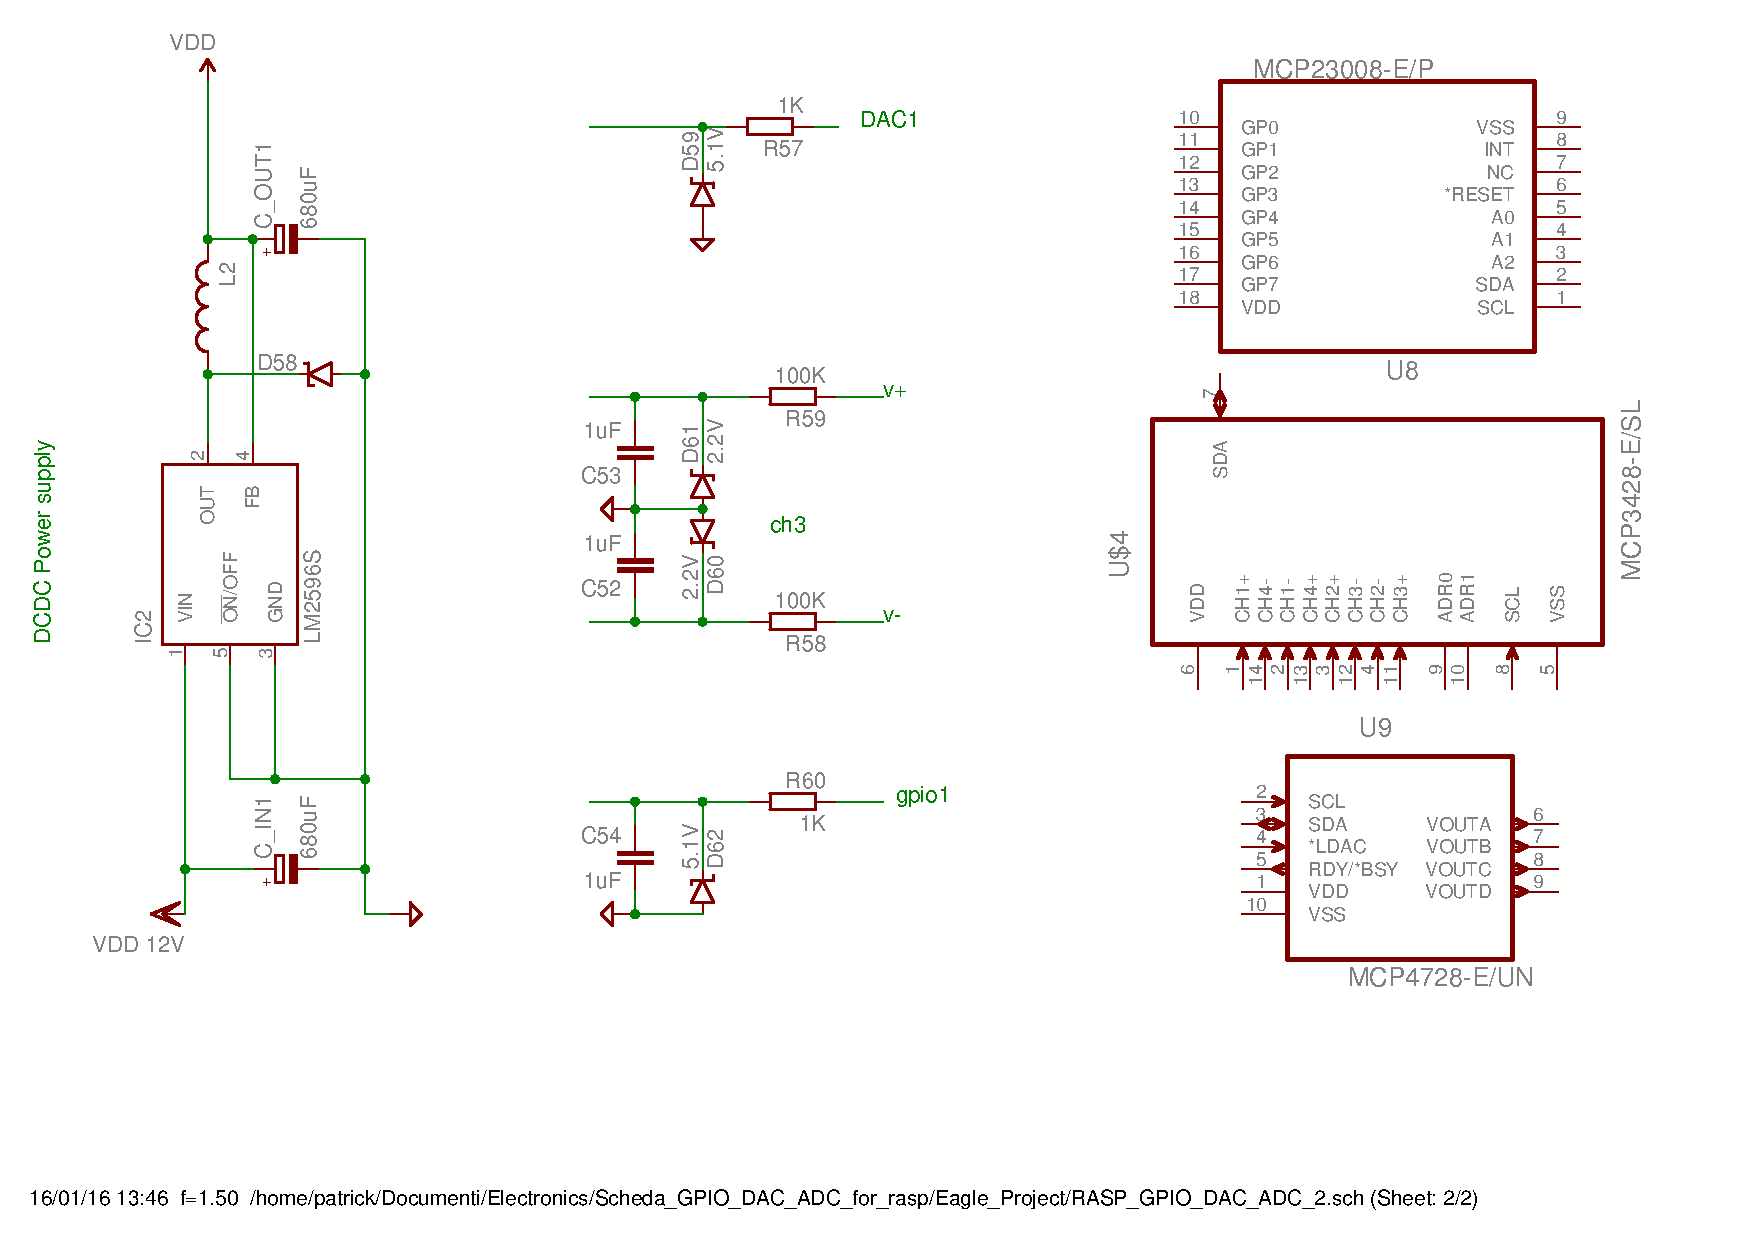
\includepdf[pages={1},noautoscale=true, offset=0 0,angle=-90]{../PDF_generated/RASP_GPIO_DAC_ADC_PARTS}

\end{document}
